\section{OCTree}
\label{theory-octree}

\subsection{Point location with respect to a plane}

Assume that a plane is given by 3 coordinates $\vec{a}, \vec{b}, \vec{c}$, and we would like to check on which side of this plane the point $\vec{p}$ is. This is uniquely given by a function
\begin{equation}
\label{equation-point-plane-test}
	ptest(\vec{a}, \vec{b}, \vec{c}, \vec{p}) = \mathrm{sgn} \{ \det (\vec{a} - \vec{p}, \vec{b} - \vec{p}, \vec{c} - \vec{p}) \}
\end{equation}
\noindent
This function takes values $1,-1$ for corresponding sides of the plane, and $0$ if the point is on the plane.

\subsection{Locating the element the given global coordinate belongs to}
\label{subsection-locating-element}

\noindent
Current convention: loop over all elements in the mesh, check if the point is inside the element using the method below. \\


\noindent
This method has $O(1)$ initialization cost, but $O(N) * ins$ query cost, which becomes wastefully slow as the number of points to locate grows. Here $ins$ is the cost of $is\_inside$ method, which has constant complexity if the query point is far away from the triangle, but requires an iterative method for nearby methods.

\noindent
There are two ways one can implement the above idea: \\
\textbf{First method:}
\begin{enumerate}
	\item Iterate over all elements, use linear $check\_inside()$
	\item For the element for which linear $check\_inside() = true$ run the nonlinear $check\_inside()$
	\item If the nonlinear $check\_inside() = false$, recursively do nonlinear $check\_inside()$ on the neighbors of the element.
\end{enumerate}
\textbf{Second method:}
\begin{enumerate}
	\item Iterate over all elements, use nonlinear $check\_inside()$
\end{enumerate}
\noindent
The first method is better, because it will on average have less runs of the iterative method, as if the point is located in a linear element, it has high probability of being located inside the nonlinear element with the same corners. \\

\noindent
An improvement would be to implement an OCTree, which will have a recursively-refined cubic mesh over the tetrahedral one, and upon initialization would place each of the tetrahedrons recursively within one or more leafs of the tree. Thus the initialization cost would be $O(N \log(N))$, and the cost of a single query $O(\log(N)) + M * inc$, where $M$ is the number of neighbors an element has. This is a considerable improvement for large number of queries. \\

\noindent
\textbf{OCTree method}:
\begin{enumerate}
	\item Construct the OCTree - grid the domain, build the hierarchical tree, place the correct element labels into each leaf
	\item For each query, locate the leaf the query point corresponds to
	\item Proceed by using one of the above methods on the element set of the leaf
\end{enumerate}

\begin{figure}[hp]
    \centering
    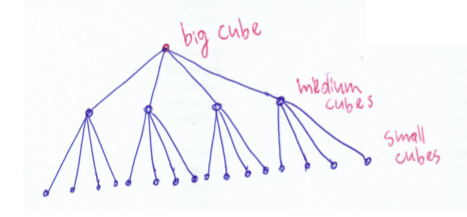
\includegraphics[scale=0.7]{doc-pics/pic-octree-3.png}
	\caption{OcTree internal structure}    
    
    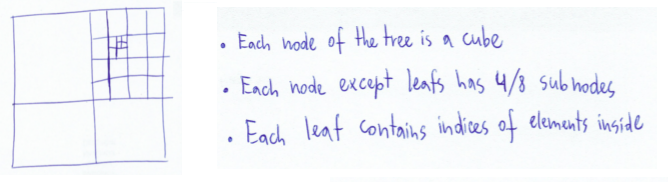
\includegraphics[scale=0.7]{doc-pics/pic-octree-1.png}
	\caption{OcTree grid}    
	
    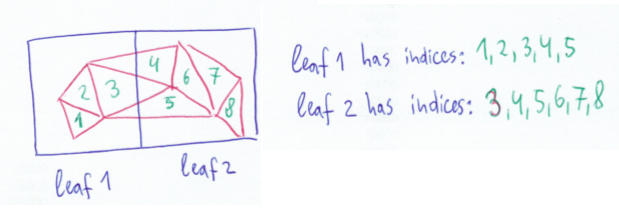
\includegraphics[scale=0.7]{doc-pics/pic-octree-2.png}
	\caption{OcTree partition of elements}    
    %\caption{Awesome Image}
    %\label{fig:awesome_image}
\end{figure}


\noindent
How does this work with parallel processing?

\subsection{Checking if a global coordinate is inside a given element (straight sided)}
\label{subsection-isinside-linear}

\noindent
For straight-sided elements the conversion between global and local coordinates is 1-to-1 in the whole space.
Therefore, it is sufficient to find the corresponding local coordinate and use the $referenceelement$ method $checkInside$. \\

\noindent
For example, for a simplex the $is\_inside(u,v,w)$ for local coordinates $(u,v,w)$ looks like 
\[u \geq 0\ \&\ v \geq 0\ \&\ w \geq 0,\ \&\ u+v+w \leq 0. \]

\noindent
Naturally, the global-local map has a finite precision, therefore the $checkInside$ method corrects for that by having a small tolerance for above inequalities, thus avoiding the case where a boundary point would be considered outside both neighboring elements because of numerical errors.


\subsection{Checking if a global coordinate is inside a given element (curvilinear elements)}
\label{subsection-isinside-nonlinear}

\noindent
This method is only defined if ($(dim_{elem} = dim_{world})$). For discussion see the $local()$ method discussion.

\noindent
In principle, this method requires an iterative solver, but first we run two simpler tests which immediately identify some of the points inside or outside of the element. \\

\noindent
\textbf{Far-point test}:
\begin{enumerate}
	\item Define linear center $\vec{p}_{CoM}$ of an element as the center of mass of its corners.
	\item Define the radius of an element $R$ as the largest distance between $\vec{p}_{CoM}$ and a point $\vec{p}_b$ on its boundary
	\item Define linear radius $R_{lin}$ to be the largest distance between $\vec{p}_{CoM}$ and one of the corners of the element. It can be shown that $R_{lin} = \frac{\sqrt{dim^2 + dim - 1}}{dim + 1} $, which is $\{ \frac{1}{2}, \frac{\sqrt{5}}{3}, \frac{\sqrt{11}}{4} \}$ for dimensions $\{1,2,3\}$.
	\item Demand that for all sensible curvilinear elements, $R$ should be bounded by some scaling of $R_{lin}$. For example, we can require that $R \leq 2 R_{lin}$, which would mean that all poins of every element should be entirely contained within $2 R_{lin}$ of its center. A more precise prefactor could be calculated from curvature constants of the bounaries of the element (max over the boundary of some expr. involving derivatives of interpolatory polynomials).
	\item Thus, if $|\vec{p}_{CoM} - \vec{p}|_2 > 2 R_{lin}$, we can immediately report that $\vec{p}$ is outside the element.
\end{enumerate}

\noindent
\textbf{Global Barycentric Coordinate test}:
\begin{enumerate}
	\item Define a global barycentric coordinate as the area enclosed by one curved boundary of the element, the point of interest, and the straight-sided boundaries that connect the point of interest and the corners of the curved boundary.
		\subitem - for 2D triangle, a barycentric coordinate is given by
		\[B = \frac{1}{2}\int_0^1 (\vec{p}(u) - \vec{p}_0) \times \partial_u \vec{p}(u) du\]
		as derived from triangle area $S = \frac{1}{2} \vec{a} \times \vec{b}$. Here $\vec{p}_0$ is the coordinate of interest.
		\subitem - for 3D tetrahedron, a barycentric coordinate is given by
		\[B = \frac{1}{3}\int_0^1 \int_0^{1-u} (\vec{p}(u,v) - \vec{p}_0) \cdot (\partial_u \vec{p}(u,v) \times \partial_v \vec{p}(u,v)) du\]
		as derived from tetrahedron volume area $V = \frac{1}{6} \vec{a} \cdot (\vec{b} \times \vec{c})$.
		Note that there is an additional factor of 2 in the barycentric equation, because triangular grid only covers half of the triangle, whereas
		parallelogram grid covers the whole (check figure \ref{fig:barycentric_coordinate_calculation})

\begin{figure}[!htb]
    \centering	
    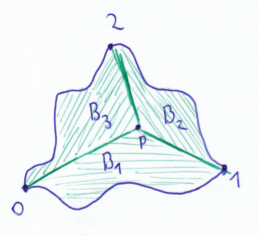
\includegraphics[scale=0.7]{doc-pics/pic-barycentric-curvilinear-definition.png}
    \caption{Definition of Barycentric Curvilinear Coordinates}
    %\label{fig:awesome_image}
\end{figure}

	\item For linear elements, the sum of barycentric coordinates always equals the total volume of the element for internal points, and is larger than that for external points. This is not true for non-convex elements, as the sum may be larger than the volume even for internal points. The method can not be improved by considering the sign of the barycentric coordinate based on the orientation of the boundary, as it is the same for internal and external points of the concave surface.
	\item Thus, if the sum of global barycentric coordinates is equal to the volume of the element, the point is automatically inside the element, otherwise we remain uncertain.
			
\end{enumerate}

\begin{figure}[!htb]
    \centering	
    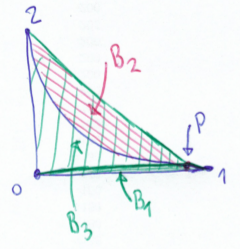
\includegraphics[scale=0.7]{doc-pics/pic-barycentric-problem-1.png}
    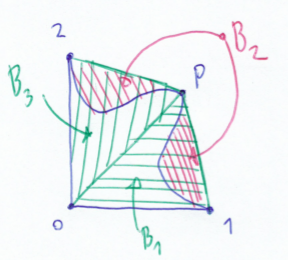
\includegraphics[scale=0.7]{doc-pics/pic-barycentric-problem-2.png}
    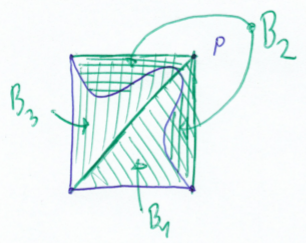
\includegraphics[scale=0.7]{doc-pics/pic-barycentric-problem-3.png}
    \caption{Problem cases with Barycentric Curvilinear coordinates}
    %\label{fig:awesome_image}
\end{figure}

\noindent
If both the above tests do not give a conclusive result, we need to use Global-To-Local mapping, and then $checkInside$ for the local coordinate. The challenges of this approach are described in the corresponding section. \\

\noindent
\textbf{Current Implementation: } There is no $is\_inside()$ method, only $local()$ method. Local method returns false if the point is not inside the element, and returns true and the correct local coordinate if it is. If the answer is true, we have to calculate the local coordinate anyway to make sure, makes sense to return it not to calculate it twice.

\begin{figure}[p]
    \centering
    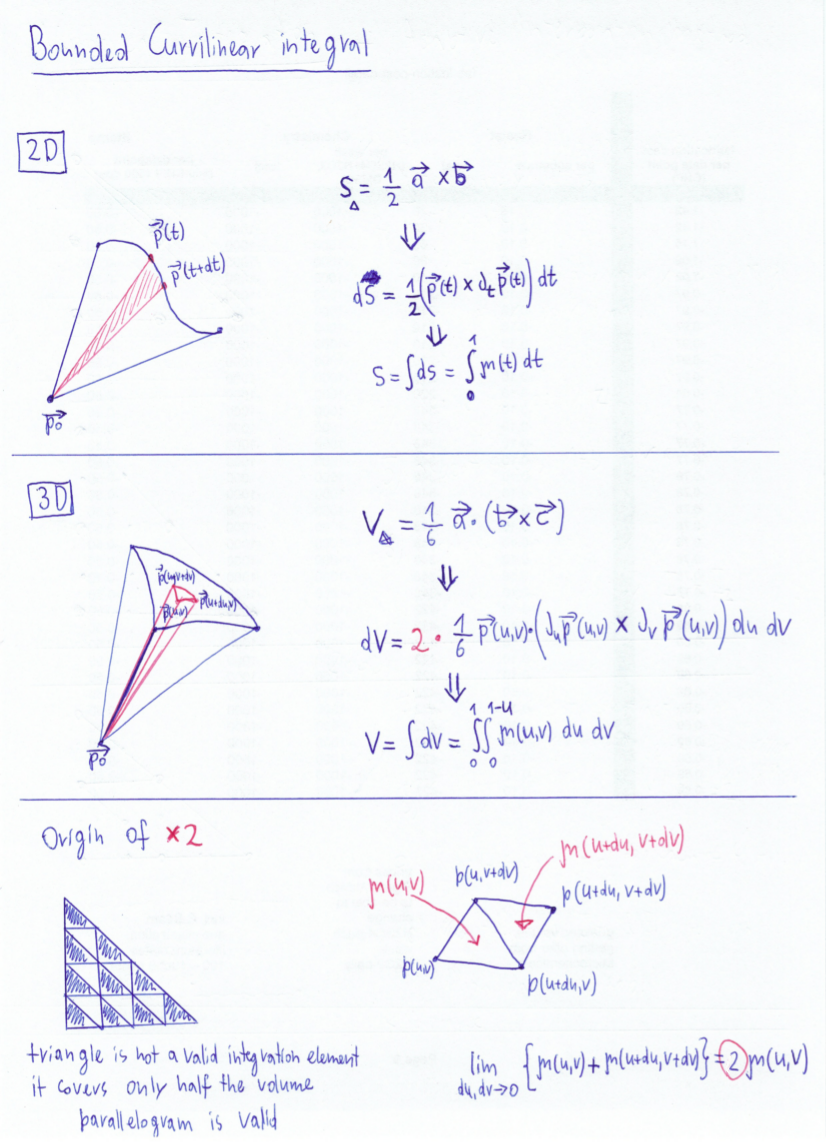
\includegraphics[scale=0.7]{doc-pics/pic-bounded-curvilinear-integral.png}
    \caption{Barycentric Coordinate Calculation}
    \label{fig:barycentric_coordinate_calculation}
\end{figure}